\documentclass[a4paper, table]{article}
% Useful packages, sorted so packages of similar functionality are grouped together. Not all are essential to make the document work, however an effort was made to make this list as minimalistic as possible. Feel free to add your own!

% Essential for making this template work are graphicx, float, tabularx, tabu, tocbibind, titlesec, fancyhdr, xcolor and tikz.

% Not essential, but you will have to debug the document a little bit when removing them are amsmath, amsthm, amssymb, amsfonts, caption, subcaption, appendix, enumitem, hyperref and cleveref.

% inputenc, lipsum, booktabs, geometry and microtype are not required, but nice to have.

\usepackage[utf8]{inputenc} % Allows the use of some special characters
\usepackage{amsmath, amsthm, amssymb, amsfonts} % Nicer mathematical typesetting
\usepackage{lipsum} % Creates dummy text lorem ipsum to showcase typsetting

\usepackage{graphicx} % Allows the use of \begin{figure} and \includegraphics
\usepackage{float} % Useful for specifying the location of a figure ([H] for ex.)
\usepackage{caption} % Adds additional customization for (figure) captions
\usepackage{subcaption} % Needed to create sub-figures

\usepackage{tabularx} % Adds additional customization for tables
\usepackage{tabu} % Adds additional customization for tables
\usepackage{booktabs} % For generally nicer looking tables

\usepackage[nottoc,numbib]{tocbibind} % Automatically adds bibliography to ToC
\usepackage[margin = 2.5cm]{geometry} % Allows for custom (wider) margins
\usepackage{microtype} % Slightly loosens margin restrictions for nicer spacing
\usepackage{titlesec} % Used to create custom section and subsection titles
\usepackage{titletoc} % Used to create a custom ToC
\usepackage{appendix} % Any chapter after \appendix is given a letter as index
\usepackage{fancyhdr} % Adds customization for headers and footers
\usepackage[shortlabels]{enumitem} % Adds additional customization for itemize.

\usepackage{hyperref} % Allows links and makes references and the ToC clickable
\usepackage[noabbrev, capitalise]{cleveref} % Easier referencing using \cref{<label>} instead of \ref{}

\usepackage{xcolor} % Predefines additional colors and allows user defined colors

\usepackage{tikz} % Useful for drawing images, used for creating the frontpage
\usetikzlibrary{positioning} % Additional library for relative positioning
\usetikzlibrary{calc} % Additional library for calculating within tikz

\usepackage[fontset=none]{ctex}

\setCJKmainfont{Source Han Serif SC}[
    BoldFont={Source Han Serif SC Bold},
    ItalicFont={KaiTi}
]

\setCJKsansfont{Source Han Sans SC}[
    BoldFont={Source Han Sans SC Medium}
]

% \setCJKmonofont[font features]{font name}


\usepackage{indentfirst}

\usepackage{listings} % for code in doc
\usepackage{pdfpages} % for inserting pdf pages
\usepackage{multirow} % as it says, for multi row in tabular
\usepackage[htt]{hyphenat} % break texttt
\usepackage{adjustbox} 

% Defines a command used by tikz to calculate some coordinates for the front-page
\makeatletter
\newcommand{\gettikzxy}[3]{%
    \tikz@scan@one@point\pgfutil@firstofone#1\relax
    \edef#2{\the\pgf@x}%
    \edef#3{\the\pgf@y}%
}
\makeatother



 % Loads in the preamble
% Give your report a title
\newcommand\reporttitle{计算机组成原理实验指导书}

% Insert course code, name, quartile number and year (or any other subtitle)
\newcommand\reportsubtitle{
    2025, Fall
}

% Add your group number (for DBL) or any other text.
%\newcommand\groupnumber{
%    \textbf{Group 0}
%}

% Insert authors and student numbers here
\newcommand\reportauthors{
    计算机组成原理课程组 \\
}

% Add the name of your tutor (for DBL) or any other text.
\newcommand\grouptutor{
    Tutor: Name Surname
}

% Date and location (default: current date and Eindhoven)
\newcommand\placeanddate{
    USTB, \today
}

% Define Ustb-blue (color of the TU/e logo). Can be changed to drastically change the look of the template
%\definecolor{Ustb-blue}{RGB}{199, 25, 24}
\definecolor{Ustb-blue}{RGB}{44, 84, 149}

% All of the following code can be removed to be left with (close to) default LaTeX behaviour.

% Sets up hyperlinks in the document to be colored
\hypersetup{
    colorlinks=true,
    linkcolor=Ustb-blue,
    urlcolor=Ustb-blue,
    citecolor = Ustb-blue
}
\urlstyle{same} % Defines settings for link and reference formatting


% Change bullet style for level 1, 2 and 3 respectively for itemize
\renewcommand{\labelitemi}{\scriptsize\textcolor{Ustb-blue}{$\blacksquare$}}% level 1
\renewcommand{\labelitemii}{\scriptsize\textcolor{Ustb-blue}{$\square$}}% level 2
\renewcommand{\labelitemiii}{\textcolor{Ustb-blue}{$\circ$}}% level 3

% \renewcommand{\labelitemi}{\small\textcolor{Ustb-blue}{\ding{70}}} % level 1
% \renewcommand{\labelitemii}{\small\textcolor{Ustb-blue}{\ding{71}}}% level 2
% \renewcommand{\labelitemiii}{\tiny\textcolor{Ustb-blue}{\ding{71}}}% level 3

% Change bullet style for level 1, 2 and 3 respectively for enumerate
\renewcommand{\labelenumi}{\textbf{\textcolor{Ustb-blue}{\arabic*.}}}% level 1
\renewcommand{\labelenumii}{\textbf{\textcolor{Ustb-blue}{[\alph*]}}}% level 2
\renewcommand{\labelenumiii}{\textbf{\textcolor{Ustb-blue}{\roman*.}}}% level 3

% Have reference labels be linked to section (section 3 will have fig. 3.1 etc.)
\counterwithin{equation}{section} % For equations
\counterwithin{figure}{section} % For figures
\counterwithin{table}{section} % For tables

% Creates a beautiful header/footer
\pagestyle{fancy}
\lhead{
\includegraphics[height = 8pt]{Figures/0. General/ustb_logo_blue_small.pdf}}
\rhead{\reporttitle}
\renewcommand{\footrulewidth}{0.4pt}
\cfoot{Page \thepage}

% Formats section, subsection and subsubsection titles respectively
\titleformat{\section}{\sffamily\color{Ustb-blue}\Large\bfseries}{\thesection\enskip\color{gray}\textbar\enskip}{0cm}{} % Formats section titles

\titleformat{\subsection}{\sffamily\color{Ustb-blue}\large\bfseries}{\thesubsection\enskip\color{gray}\textbar\enskip}{0cm}{} % Formats subsection titles

\titleformat{\subsubsection}{\sffamily\color{Ustb-blue}\bfseries}{\thesubsubsection\enskip\color{gray}\textbar\enskip}{0cm}{} % Formats subsubsection titles

% Formats captions
\DeclareCaptionFont{Ustb-blue}{\color{Ustb-blue}}
\captionsetup{labelfont={Ustb-blue,bf}}

% Changes font to mlmodern
\usepackage{mlmodern}
\usepackage{color}
\usepackage{graphicx}

% Removes indent when starting a new paragraph
\setlength\parindent{0pt}

% Limits the ToC to sections and subsections (no subsubsec.)
\setcounter{tocdepth}{2}

\setlength{\parindent}{2em}

\setmonofont{Fira Code}

\lstset{
    language=Verilog,
    backgroundcolor = \color{Ustb-blue!10},    % 背景色:淡黄
    basicstyle = \small\ttfamily,           % 基本样式 + 小号字体
    rulesepcolor= \color{gray},             % 代码块边框颜色
    breaklines = true,                  % 代码过长则换行
    numbers = left,                     % 行号在左侧显示
    numberstyle = \small,               % 行号字体
    keywordstyle = \color{Ustb-blue}\textbf,            % 关键字颜色
    commentstyle =\color{purple},        % 注释颜色
    stringstyle = \color{Ustb-blue!50!purple},          % 字符串颜色
    frame = shadowbox,                  % 用(带影子效果)方框框住代码块
    showspaces = false,                 % 不显示空格
    columns = fixed,                    % 字间距固定
    morekeywords = {as},                % 自加新的关键字(必须前后都是空格)
    deletendkeywords = {compile}        % 删除内定关键字;删除错误标记的关键字用deletekeywords删!
}

\newcommand{\foreword}[4]{
    \begin{minipage}[l]{0.4\textwidth}
        \textit{\textcolor{Ustb-blue}{\Large #1}}\normalsize \textit{(#2)}\\
        {\small\textit{#3}}
    \end{minipage}
    \hfill
    \begin{minipage}[r]{0.55\textwidth}
        \begin{flushright}
            \includegraphics[width=.9\textwidth]{#4}
        \end{flushright}
    \end{minipage}
    \vspace{1em}
    \textcolor{gray}{\[\sim \cdot \sim\]}
    \vspace{1em}
}

\newcommand{\highlight}[1]{
    \textbf{\textcolor{Ustb-blue}{#1}}
}

\setcounter{tocdepth}{4}
\setcounter{secnumdepth}{3} % Loads in user defined settings


\begin{document}
\setcounter{section}{-1}
% Inserts the front page
\begin{titlepage}

    \centering

    \begin{tikzpicture}

        \node[opacity=0.3,inner sep=0pt,remember picture,overlay] at (4.5,-0.5){
\includegraphics[width= 0.8 \textwidth]{Figures/0. General/ustb_logo_gray.pdf}};

        \node[inner sep=0pt] (logo) at (0,0)
        {
\includegraphics[width=.25\textwidth]{Figures/0. General/ustb_logo_blue_small.pdf}};

        \node[text width = 0.5\textwidth, right = of logo](title){\sffamily\huge\reporttitle};

        \node[text width = 0.5\textwidth, yshift = 0.75cm, below = of title](subtitle){\sffamily\Large \reportsubtitle};

        \gettikzxy{(subtitle.south)}{\sffamily\subtitlex}{\subtitley}
        \gettikzxy{(title.north)}{\titlex}{\titley}
        \draw[line width=1mm, Ustb-blue]($(logo.east)!0.5!(title.west)$) +(0,\subtitley) -- +(0,\titley);

    \end{tikzpicture}
    \vspace{3cm}

    % \sffamily\groupnumber

    \begin{table}[H]
        \centering
        \sffamily
        \large
        \begin{tabu} to 0.8\linewidth {cc}
            \textbf{作者} \\
            \hline

            \sffamily\reportauthors
        \end{tabu}

    \end{table}

    %    \sffamily \grouptutor

    \tikz[remember picture,overlay]\node[anchor=south,inner sep=0pt] at (current page.south) {
\includegraphics[width=\paperwidth]{Figures/0. General/ustb.pdf}};

    \mbox{}
    \vfill
    \sffamily \Large \textcolor{white}{\placeanddate} \\



\end{titlepage}

\cleardoublepage

% Generates a ToC without page number
{\hypersetup{linkcolor=black} % Keeps the ToC black even with non-black linkcolor
    \tableofcontents\thispagestyle{empty}}
\cleardoublepage

% contains inspiration for formatting tables, images, text citations etc.
%    \section{This is a section} \pagenumbering{roman}
\subsection{This is a subsection}

\subsubsection{This is a subsubsection}
This section contains some templates that can be used to create a uniform style within the document. It also shows of the overall formatting of the template, created using the predefined styles from the \texttt{settings.tex} file.

\subsection{General formatting}
Firstly, the document uses the font mlmodern, using no indent for new paragraphs and commonly uses the color \textcolor{Ustb-blue}{Ustb-blue} (the color of the TU/e logo) in its formatting. It uses the \texttt{fancyhdr} package for its headers and footers, using the TU/e logo and report title as the header and the page number as the footer. The template uses custom section, subsection and subsubsection formatting making use of the \texttt{titlesec} package.\\
The \texttt{hyperref} package is responsible for highlighting and formatting references like figures and tables. For example \cref{table: style 1} or \cref{fig: three images}. It also works for citations \cite{texbook}. Note how figure numbers are numbered according to the format \texttt{<chapter number>.<figure number>}.\\

Bullet lists are also changed globally, for a maximum of 3 levels:

\begin{itemize}
    \item Item 1
    \item Item 2
          \begin{itemize}
              \item subitem 1
                    \begin{itemize}
                        \item subsubitem 1
                        \item subsubitem 2
                    \end{itemize}
          \end{itemize}
    \item Item 3
\end{itemize}

Similarly numbered lists are also changed document wide:

\begin{enumerate}
    \item Item 1
    \item Item 2
          \begin{enumerate}
              \item subitem 1
                    \begin{enumerate}
                        \item subsubitem 1
                        \item subsubitem 2
                    \end{enumerate}
          \end{enumerate}
    \item Item 3
\end{enumerate}

\newpage

\subsection{Tables and figures}
The following table, \cref{table: style 1}, shows a possible format for tables in this document. Alternatively, one can also use the black and white version of this, shown in \cref{table: style 2}. Note that caption labels are in the format \textbf{\textcolor{Ustb-blue}{Table x.y:} }
\begin{table}[ht]
    \rowcolors{2}{Ustb-blue!10}{white}
    \centering
    \caption{A table without vertical lines.}
    \begin{tabular}[t]{ccccc}
        \toprule
        \color{Ustb-blue}\textbf{Column 1} & \color{Ustb-blue}\textbf{Column 2} & \color{Ustb-blue}\textbf{Column 3} & \color{Ustb-blue}\textbf{Column 4} & \color{Ustb-blue}\textbf{Column 5} \\
        \midrule
        Entry 1                            & 1                                  & 2                                  & 3                                  & 4                                  \\
        Entry 2                            & 1                                  & 2                                  & 3                                  & 4                                  \\
        Entry 3                            & 1                                  & 2                                  & 3                                  & 4                                  \\
        Entry 4                            & 1                                  & 2                                  & 3                                  & 4                                  \\
        \bottomrule
    \end{tabular}
    \label{table: style 1}
\end{table}

\begin{table}[ht]
    \rowcolors{2}{gray!10}{white}
    \centering
    \caption{A table without vertical lines.}
    \begin{tabular}[t]{ccccc}
        \toprule
        \textbf{Column 1} & \textbf{Column 2} & \textbf{Column 3} & \textbf{Column 4} & \textbf{Column 5} \\
        \midrule
        Entry 1           & 1                 & 2                 & 3                 & 4                 \\
        Entry 2           & 1                 & 2                 & 3                 & 4                 \\
        Entry 3           & 1                 & 2                 & 3                 & 4                 \\
        Entry 4           & 1                 & 2                 & 3                 & 4                 \\
        \bottomrule
    \end{tabular}
    \label{table: style 2}
\end{table}

For normal, single image figures, the standard \texttt{\textbackslash begin\{figure\}} environment can be used. For multi-image figures, one could use either the \texttt{\textbackslash begin\{subfigure\}} environment to get a main caption with 3 subcaptions like \cref{fig: three images} or the \texttt{\textbackslash begin\{minipage\}} environment to get 3 independent captions like \cref{fig: style 2 image a} - \ref{fig: style 2 image c}

\begin{figure}[H]
    \centering
    \begin{subfigure}[b]{0.3\textwidth}
        \centering
        \includegraphics[width=\textwidth]{example-image-a}
        \caption{image a}
        \label{fig: style 1 image a}
    \end{subfigure}
    \hfill
    \begin{subfigure}[b]{0.3\textwidth}
        \centering
        \includegraphics[width=\textwidth]{example-image-b}
        \caption{image b}
        \label{fig: style 1 image b}
    \end{subfigure}
    \hfill
    \begin{subfigure}[b]{0.3\textwidth}
        \centering
        \includegraphics[width=\textwidth]{example-image-c}
        \caption{image c}
        \label{fig: style 1 image c}
    \end{subfigure}
    \caption{Three images}
    \label{fig: three images}
\end{figure}

\begin{figure}[H]
    \centering
    \begin{minipage}{0.3\textwidth}
        \centering
        \includegraphics[width=\textwidth]{example-image-a}
        \captionof{figure}{image a}
        \label{fig: style 2 image a}
    \end{minipage}
    \hfill
    \begin{minipage}{0.3\textwidth}
        \centering
        \includegraphics[width=\textwidth]{example-image-b}
        \captionof{figure}{image b}
        \label{fig: style 2 image b}
    \end{minipage}
    \hfill
    \begin{minipage}{0.3\textwidth}
        \centering
        \includegraphics[width=\textwidth]{example-image-c}
        \captionof{figure}{image c}
        \label{fig: style 2 image c}
    \end{minipage}
\end{figure} % Feel free to remove / comment out
%    \cleardoublepage

% Generates a list of symbols table
% \section*{list of symbols} \label{section: symbols}

\begin{table}[ht]
    \rowcolors{2}{gray!10}{white}
    \centering
    \caption{list of symbols}
    \begin{tabular}[t]
        {m{0.15\textwidth}m{0.15\textwidth}m{0.65\textwidth}}
        \toprule
        \textbf{实验}               & \textbf{实验编号} & \textbf{实验名称}            \\
        \midrule
        \multirow{3}{*}{\ref{lab1}} & \ref{sss: lab1.1} & Vivado 设计流程学习          \\
                                    & \ref{sss: lab1.2} & Vivado 设计流程练习 – 流水灯 \\
                                    & \ref{sss: lab1.3} & Vivado 代码编辑和RTL分析     \\
        \bottomrule
    \end{tabular}
\end{table}
% \cleardoublepage

% Creates the introduction, starting page numbering
\section{写在前面} \label{section: introduction}

\foreword{
    第一步
}{
    文森特·梵·高
}{
    人们经常会忘记的是,纵使是一趟没有目的地的旅程,也还是从单纯踏出第一步开始的。
}{
    Figures/C0.jpg
}

\begin{flushright}
    The machine is cold, but COAT is warm.

    \highlight{Computer Organization and Architecture Tutorial}

    Welcome to the digital world!
\end{flushright}

\vspace*{2em}

计算机组成原理课程,作为计算机专业的基础课,是计算机专业的使用者理解计算机构成的原理和学会用好计算机的关键。在这门课程当中,你会了解到一个基本的计算机系统是如何构成,了解到软件程序与硬件交互,更进一步地了解计算机系统背后的原理。

\subsection{关于RTFM, STFW, RTFSC}

在学习的过程中,你会使用到我们提供的处理器开发环境,其中包括了对基本的处理器的仿真验证和综合上板的功能。在这一过程中,你可能会遇到一些错误,这些错误,
有些可能是由于你对实验内容的不够了解,有些可能是因为你对实验环境提供的工具甚至是实验环境本身的不了解,这些问题不仅是在实验当中,也可能存在于大家未来的学习和工作当中,基于此,我们在这里向大家介绍计算机专业前辈们总结出对付错误的经验。

\paragraph{\bfseries RTFM} 阅读手册。在本实验中提供的手册有很多,比如实验指导书,比如说关于指令集架构的文档。如果你遇到错误,请首先先翻一翻手册,
看看是否是因为手册中某个没有注意到细节而导致了错误。手册会对实验环境和实验内容进行简要的介绍,它无法覆盖实验中的方方面面,
但是一定会将实验中的重点难点展现给大家,因此查询手册往往能够帮助我们快速解决问题。我们会在后面的资源使用路线中简单介绍一下本课程中可能会用到的各手册的内容。

\paragraph{\bfseries STFW} 上网搜索。手册会尽量将实验中的细节描述清楚,帮助大家完成实验。然而遗憾的是,手册没有办法覆盖到实验中的每一个细节,每一种可能的错误,
(比如大魔王Vivado的各种报错)所以这种时候可以考虑上网搜索。从效率的角度考虑,我们希望大家尽量使用Google/Bing 国际版进行搜索,多在国外的一些优秀论坛上寻找解决方案。

\paragraph{\bfseries RTFSC} 阅读源代码。实验环境中有大量代码,他们是整个实验环境的支撑。想要完成好实验,一定需要充分的了解实验环境,手册中已经给出了一部分关于实验环境的描述,
但是并不足以支持你理解实验环境的全貌,所以适当的阅读实验环境中的源代码,诸如测试用例的源代码,仿真环境的源代码,通过阅读这些代码,相信你不仅能解决问题,也能加深自己对于整个实验环境的理解。

当自己已经充分尝试过以上方法时,你可以向助教,老师,或者是其他同学求助,但是希望你在提问的过程中,能够尽量清晰的描述你的问题,帮助你提问的人能够更快理解你当前所面对的情况,更好的解决问题。

关于如何提问,你可以阅读《提问的智慧》或《别像弱智一样提问》,上面的三板斧和正确提问的方法是计算机世界的答案之书,在本门课程的理论内容的学习之外,我更希望大家能够学会正确的提问,学会正确而高效的寻找答案的方法。 \pagenumbering{arabic}
\cleardoublepage

% Copy this to add more chapters
\section{不考虑冲突的简单五级流水划分}\label{lab1}

\foreword{
    有橡树的风景
}{
    亚历山德拉·卡拉梅
}{
    树干总是一成不变,枝叶却纷披而伸展。
}{
    Figures/C8.jpg
}

\subsection{流水级介绍}

在计组理论课上大家已经了解过了流水级的概念,不在这里进行过多的解释。在理想情况下,无阻塞的流水级每周期处理一条指令,相比较于单周期CPU效率能够有显著的提升。

但是很多时候流水级会被阻塞,这就意味着如果如果后面的流水级被阻塞,前面的流水级也立即需要被阻塞。因为此时的后面流水级不通,系统不能接受新的数据,所有前面的流水级必须将原有的数据留在本流水级,否则会导致数据的丢失。

我们在实验中采用的策略是:

给每个流水级都安排一个``管理人员'',能与前后级的管理人员进行互相的沟通交流。他会向后一级发送``下个时刻我有东西给你''的请求,同时向前一级发送``下一个时刻我可以接受你传递来的东西'',这样子每级串联起来环环相扣。给出一个示例的设计代码:

\begin{lstlisting}
    module stallable_pipeline #(
        parameter WIDTH = 32
    ) (
        input wire clk,
        input wire resetn,
        input wire validin,
        input wire [WIDTH-1:0] datain,
        input wire out_allow,
        output wire validout,
        output wire [WIDTH-1:0] dataout
    );
    reg [WIDTH-1:0] pipe1_data;
    reg [WIDTH-1:0] pipe2_data;
    reg [WIDTH-1:0] pipe3_data;
    reg pipe1_valid;
    reg pipe2_valid;
    reg pipe3_valid;

    wire pipe1_allowin;
    wire pipe1_ready_go;
    wire pipe1_to_pipe2_valid;
    assign pipe1_ready_go = ......;
    assign pipe1_allowin = ~pipe1_valid || pipe1_ready_go & pipe2_allowin;
    assign pipe1_to_pipe2_valid = pipe1_valid & pipe1_ready_go;

    always @(posedge clk) begin
        if (~resetn) begin  // 复位使得该触发器数据无效
        pipe1_valid <= 1'b0;
        end else if (pipe1_allowin) begin
        pipe1_valid <= validin;
        end

        if (pipe1_allowin & validin) begin
        pipe1_data <= datain;
        end
    end

    wire pipe2_allowin;
    wire pipe2_ready_go;
    wire pipe2_to_pipe3_valid;
    assign pipe2_ready_go = ......;
    assign pipe2_allowin = ~pipe2_valid || pipe2_ready_go & pipe3_allowin;
    assign pipe2_to_pipe3_valid = pipe2_valid & pipe2_ready_go;

    always @(posedge clk) begin
        if (~resetn) begin
        pipe2_valid <= 1'b0;
        end else if (pipe2_allowin) begin
        pipe2_valid <= pipe1_to_pipe2_valid;
        end
        if (pipe2_allowin & pipe1_to_pipe2_valid) begin
        pipe2_data <= pipe1_data;
        end
    end

    wire pipe3_allowin;
    wire pipe3_ready_go;
    wire pipe3_to_out_valid;  //赋值给validout
    assign pipe3_ready_go = ......;
    assign pipe3_allowin = ~pipe3_valid || pipe3_ready_go & out_allow;
    assign pipe3_to_out_valid = pipe3_valid & pipe3_ready_go;

    always @(posedge clk) begin
        if (~resetn) begin
        pipe3_valid <= 1'b0;
        end else if (pipe3_allowin) begin
        pipe3_valid <= pipe2_to_pipe3_valid;
        end
        if (pipe3_allowin & pipe2_to_pipe3_valid) begin
        pipe3_data <= pipe2_data;
        end
    end
    assign validout = pipe3_to_out_valid;
    assign dataout  = pipe3_data;
    endmodule
\end{lstlisting}


下面对些许信号进行解释:

\texttt{pipex\_valid}表示为第\texttt{x}级的有效位,使用触发器实现,为1的时候表示当前时钟周期时的数据有效,好处在于,当我们需要将流水线清空的时候,不需要将所有\texttt{data}置为0,只需要将\texttt{valid}设为0.

\texttt{pipex\_allowin}是往前传递的信号,为1是表示当前允许接收前一级传入的数据。

\texttt{pipex\_ready\_go}表示当前拍的状态,为1时表示数据在当前级的任务已经完成,可以往后一级传递数据。

\texttt{pipex\_to\_pipex+1\_valid}向后一级传递的信号,为1表示有数据需要在下个周期传入后一级。

\subsection{单周期处理器拆分}

我们设计的是经典的单发射五级流水线划分,从前往后依次是:取值(IF),译码(ID),执行(EXE),访存(MEM),写回(WB)。

取指阶段的主要功能是将指令取回;

译码阶段的主要功能是解析指令生成控制信号并读取通用寄存器堆生成源操作数;

执行阶段的主要功能是对源操作数进行算术逻辑类指令的运算或者访存指令的地址计算;

访存阶段的主要功能是取回访存的结果;

写回阶段的主要功能是将结果写入通用寄存
器堆。

结合这个流水线阶段的划分方案,我们将之前设计的单发射 CPU 的数据通路拆分为五段,
并在各段之间加入触发器作为流水线缓存。

这里给出取指级的详细代码:

\begin{lstlisting}
    `include "mycpu_head.v"

    module IF_stage(
        input wire clk,
        input wire reset,
        input wire ds_allowin,
        input wire [`BR_BUS_WD  -1 :0] br_bus,
        output     wire             fs_to_ds_valid,
        output wire [`FS_TO_DS_BUS_WD-1 :0] fs_to_ds_bus,
        // inst sram interface
        output wire inst_sram_en,
        output wire [3:0] inst_sram_we,
        output wire [31:0] inst_sram_addr,
        output wire [31:0] inst_sram_wdata,
        input  wire [31:0] inst_sram_rdata
        );
        //if级握手信号
        reg         fs_valid; 
        wire        fs_ready_go;
        wire        fs_allowin;
        wire        to_fs_valid; 
        
        wire [31:0] seq_pc; //顺序的地址
        wire [31:0] next_pc; //下一个执行的地址,可能会跳转
        
        wire br_taken; //跳转信号
        wire [31:0] br_target;//跳转地址
        
        assign {br_taken,br_target} = br_bus; //跳转信号传递
        
        wire [31:0] fs_inst; //fs阶段的inst和pc,往后传递
        reg [31:0] fs_pc;
        
        //if向id传递的bus
        assign fs_to_ds_bus = {fs_inst,fs_pc};
        
        //pre-if stage
        assign to_fs_valid = ~reset; 
        assign seq_pc = fs_pc + 3'h4; //顺序
        assign next_pc = (br_taken == 1 ) ? br_target :seq_pc; 
        
        //IF stage
        assign fs_ready_go = 1'b1; //可以传输
        assign fs_allowin = !fs_valid || fs_ready_go && ds_allowin; //允许进入,
        assign fs_to_ds_valid = fs_valid && fs_ready_go;
        
        always@(posedge clk)begin
        if(reset)begin
        fs_valid <= 1'b0;
        end else if(fs_allowin)begin
        fs_valid <= to_fs_valid;
        end
        end
        
    always@(posedge clk)begin
        if(reset)begin
        fs_pc <= 32'h1bfffffc;
        end else if(to_fs_valid && fs_allowin)begin
        fs_pc <= next_pc;
    end
    end
    
    assign inst_sram_en = to_fs_valid && fs_allowin;   //
    assign inst_sram_we = 4'h0;  //写
    assign inst_sram_addr =next_pc; 
    assign inst_sram_wdata = 32'b0; 
    
    assign fs_inst = inst_sram_rdata; 
    
    endmodule
\end{lstlisting}

关于转移指令更新 PC ,由于转移指令需要在译码级才能知道正确的跳转方向和目标,所以我们将转移指令的pc修改时间放在译码级,此时我们应该注意,
pre-IF 阶段的 \texttt{nextpc} 生成逻辑中,来自 PC 相对转移指令跳转目标的那一支,其跳转目标计算所用的 PC 是处在译码阶段的转移指令的 PC,不是此时取指阶段的PC。

\texttt{fs\_to\_ds\_bus}存放着每一级的缓存,需要往后传递,它的位宽取决于数据内容的大小,这里通过宏定义
(\texttt{mycpu\_head.v})进行统一管理,具体如下,xx为自身传递的位宽大小,根据自身设计而定,没有强制要求:

\begin{lstlisting}
    `ifndef MYCPU_H
        `define MYCPU_H

        `define BR_BUS_WD        xx
        `define FS_TO_DS_BUS_WD  xx
        `define DS_TO_ES_BUS_WD  xx
        `define ES_TO_MS_BUS_WD  xx
        `define MS_TO_WS_BUS_WD  xx
        `define WS_TO_RF_BUS_WD  xx
    `endif
\end{lstlisting}

给出译码级的详细代码:

\begin{lstlisting}
    `include "mycpu_head.v"

    module ID_stage(
        input  wire    clk,
        input  wire    reset,
        //allowin
        input  wire    es_allowin,
        output wire    ds_allowin,
        //from if stage
        input   wire        fs_to_ds_valid,
        input wire [`FS_TO_DS_BUS_WD-1 : 0] fs_to_ds_bus,
        //to ex stage
        output  wire         ds_to_es_valid,
        output  wire [`DS_TO_ES_BUS_WD -1 : 0 ] ds_to_es_bus,
        //to if stage
        output wire  [`BR_BUS_WD -1 : 0 ] br_bus   ,
        //to rf :write back
        input  wire  [`WS_TO_RF_BUS_WD -1 :0] ws_to_rf_bus
    );

    wire br_taken;
    wire [31:0] br_target;

    wire [31:0] ds_pc;
    wire [31:0] ds_inst;

    reg         ds_valid;
    wire        ds_ready_go;

    wire [11:0] alu_op;

    wire load_op;  //加载信号
    wire src1_is_pc; //来自src为pc地址
    wire src2_is_imm; //src2为imm
    wire res_from_mem; //result来自mem
    wire dst_is_r1;
    wire gr_we; 
    wire mem_we; 
    wire src_reg_is_rd;
    wire [4:0]dest;
    wire rj_eq_rd;
    wire [31:0]rj_value;
    wire [31:0]rkd_value;
    wire [31:0]imm;
    wire [31:0]br_offs;
    wire [31:0]jirl_offs;

    //分段
    wire [5:0] op_31_26;
    wire [3:0] op_25_22;
    wire [ 1:0] op_21_20;
    wire [ 4:0] op_19_15;

    wire [ 4:0] rd;
    wire [ 4:0] rj;
    wire [ 4:0] rk;

    wire [11:0] i12;
    wire [19:0] i20;
    wire [15:0] i16;
    wire [25:0] i26;

    wire [63:0] op_31_26_d;
    wire [15:0] op_25_22_d;
    wire [ 3:0] op_21_20_d;
    wire [31:0] op_19_15_d;

    wire        inst_add_w;
    wire        inst_sub_w;
    wire        inst_slt;
    wire        inst_sltu;
    wire        inst_nor;
    wire        inst_and;
    wire        inst_or;
    wire        inst_xor;
    wire        inst_slli_w;
    wire        inst_srli_w;
    wire        inst_srai_w;
    wire        inst_addi_w;
    wire        inst_ld_w;
    wire        inst_st_w;
    wire        inst_jirl;
    wire        inst_b;
    wire        inst_bl;
    wire        inst_beq;
    wire        inst_bne;
    wire        inst_lu12i_w;

    wire        need_ui5;
    wire        need_si12;
    wire        need_si16;
    wire        need_si20;
    wire        need_si26;
    wire        src2_is_4;

    wire [ 4:0] rf_raddr1;
    wire [31:0] rf_rdata1;
    wire [ 4:0] rf_raddr2;
    wire [31:0] rf_rdata2;

    wire rf_we ; //写使能
    wire [4:0] rf_waddr;
    wire [31:0] rf_wdata;

    wire [31:0] alu_src1 ;
    wire [31:0] alu_src2;
    wire [31:0] alu_result;

    wire [31:0] mem_result;
    wire [31:0] final_result;

    assign op_31_26  = ds_inst[31:26];
    assign op_25_22  = ds_inst[25:22];
    assign op_21_20  = ds_inst[21:20];
    assign op_19_15  = ds_inst[19:15];

    assign rd   = ds_inst[ 4: 0];
    assign rj   = ds_inst[ 9: 5];
    assign rk   = ds_inst[14:10];
                
    assign i12  = ds_inst[21:10];
    assign i20  = ds_inst[24: 5];
    assign i16  = ds_inst[25:10];
    assign i26  = {ds_inst[ 9: 0], ds_inst[25:10]};

    decoder_6_64 u_dec0(.in(op_31_26 ), .out(op_31_26_d ));
    decoder_4_16 u_dec1(.in(op_25_22 ), .out(op_25_22_d ));
    decoder_2_4  u_dec2(.in(op_21_20 ), .out(op_21_20_d ));
    decoder_5_32 u_dec3(.in(op_19_15 ), .out(op_19_15_d ));

    ///////////////////////////////////
    assign inst_add_w  = op_31_26_d[6'h00] & op_25_22_d[4'h0] & op_21_20_d[2'h1] & op_19_15_d[5'h00];
    assign inst_sub_w  = op_31_26_d[6'h00] & op_25_22_d[4'h0] & op_21_20_d[2'h1] & op_19_15_d[5'h02];
    assign inst_slt    = op_31_26_d[6'h00] & op_25_22_d[4'h0] & op_21_20_d[2'h1] & op_19_15_d[5'h04];
    assign inst_sltu   = op_31_26_d[6'h00] & op_25_22_d[4'h0] & op_21_20_d[2'h1] & op_19_15_d[5'h05];
    assign inst_nor    = op_31_26_d[6'h00] & op_25_22_d[4'h0] & op_21_20_d[2'h1] & op_19_15_d[5'h08];
    assign inst_and    = op_31_26_d[6'h00] & op_25_22_d[4'h0] & op_21_20_d[2'h1] & op_19_15_d[5'h09];
    assign inst_or     = op_31_26_d[6'h00] & op_25_22_d[4'h0] & op_21_20_d[2'h1] & op_19_15_d[5'h0a];
    assign inst_xor    = op_31_26_d[6'h00] & op_25_22_d[4'h0] & op_21_20_d[2'h1] & op_19_15_d[5'h0b];
    assign inst_slli_w = op_31_26_d[6'h00] & op_25_22_d[4'h1] & op_21_20_d[2'h0] & op_19_15_d[5'h01];
    assign inst_srli_w = op_31_26_d[6'h00] & op_25_22_d[4'h1] & op_21_20_d[2'h0] & op_19_15_d[5'h09];
    assign inst_srai_w = op_31_26_d[6'h00] & op_25_22_d[4'h1] & op_21_20_d[2'h0] & op_19_15_d[5'h11];
    assign inst_addi_w = op_31_26_d[6'h00] & op_25_22_d[4'ha];
    assign inst_ld_w   = op_31_26_d[6'h0a] & op_25_22_d[4'h2];
    assign inst_st_w   = op_31_26_d[6'h0a] & op_25_22_d[4'h6];
    assign inst_jirl   = op_31_26_d[6'h13];
    assign inst_b      = op_31_26_d[6'h14];
    assign inst_bl     = op_31_26_d[6'h15];
    assign inst_beq    = op_31_26_d[6'h16];
    assign inst_bne    = op_31_26_d[6'h17];
    assign inst_lu12i_w= op_31_26_d[6'h05] & ~ds_inst[25];

    /////////////////////////////////
    assign alu_op[ 0] = inst_add_w | inst_addi_w | inst_ld_w | inst_st_w
                        | inst_jirl | inst_bl;
    assign alu_op[ 1] = inst_sub_w;
    assign alu_op[ 2] = inst_slt;
    assign alu_op[ 3] = inst_sltu;
    assign alu_op[ 4] = inst_and;
    assign alu_op[ 5] = inst_nor;
    assign alu_op[ 6] = inst_or;
    assign alu_op[ 7] = inst_xor;
    assign alu_op[ 8] = inst_slli_w;
    assign alu_op[ 9] = inst_srli_w;
    assign alu_op[10] = inst_srai_w;
    assign alu_op[11] = inst_lu12i_w;
    //信号
    assign need_ui5   =  inst_slli_w | inst_srli_w | inst_srai_w;
    assign need_si12  =  inst_addi_w | inst_ld_w | inst_st_w;
    assign need_si16  =  inst_jirl | inst_beq | inst_bne;
    assign need_si20  =  inst_lu12i_w;
    assign need_si26  =  inst_b | inst_bl;
    assign src2_is_4  =  inst_jirl | inst_bl;

    assign imm = src2_is_4 ? 32'h4                      :
                need_si20 ? {i20[19:0], 12'b0}         :
                need_ui5  ? rk                         :
                {{20{i12[11]}}, i12[11:0]} ;

    assign br_offs = need_si26 ? {{ 4{i26[25]}}, i26[25:0], 2'b0} :
                                {{14{i16[15]}}, i16[15:0], 2'b0} ;

    assign jirl_offs = {{14{i16[15]}}, i16[15:0], 2'b0};

    assign src_reg_is_rd = inst_beq | inst_bne | inst_st_w;

    assign src1_is_pc    = inst_jirl | inst_bl;

    assign src2_is_imm   = inst_slli_w |
                        inst_srli_w |
                        inst_srai_w |
                        inst_addi_w |
                        inst_ld_w   |
                        inst_st_w   |
                        inst_lu12i_w|
                        inst_jirl   |
                        inst_bl     ;

    assign res_from_mem  = inst_ld_w;
    assign dst_is_r1     = inst_bl;
    assign gr_we         = ~inst_st_w & ~inst_beq & ~inst_bne & ~inst_b ;
    assign mem_we        = inst_st_w;
    assign dest          = dst_is_r1 ? 5'd1 : rd;

    assign rf_raddr1 = rj;
    assign rf_raddr2 = src_reg_is_rd ? rd :rk;

    regfile u_regfile(
        .clk    (clk      ),
        .raddr1 (rf_raddr1),
        .rdata1 (rf_rdata1),
        .raddr2 (rf_raddr2),
        .rdata2 (rf_rdata2),
        .we     (rf_we    ),
        .waddr  (rf_waddr ),
        .wdata  (rf_wdata )
        );
        
    assign rj_value  = rf_rdata1;
    assign rkd_value = rf_rdata2;

    assign rj_eq_rd = (rj_value == rkd_value);
    assign br_taken = (   inst_beq  &&  rj_eq_rd
                    || inst_bne  && !rj_eq_rd
                    || inst_jirl
                    || inst_bl
                    || inst_b
                    ) && ds_valid;
    assign br_target = (inst_beq || inst_bne || inst_bl || inst_b) ? (ds_pc + br_offs) :
                                                    /*inst_jirl*/ (rj_value + jirl_offs);
                                                    
    assign br_bus = {br_taken , br_target};

    reg [`FS_TO_DS_BUS_WD-1 : 0] fs_to_ds_bus_r;

    assign {ds_inst,
            ds_pc} = fs_to_ds_bus_r;

    assign {rf_we, //37:37
            rf_waddr, //36:32
            rf_wdata //31:0
            } = ws_to_rf_bus;     
    
    assign ds_to_es_bus = {alu_op       ,  
                        load_op      ,  
                        src1_is_pc   ,   
                        src2_is_imm  ,  
                        src2_is_4    ,  
                        gr_we        , 
                        mem_we       ,   
                        dest         ,   
                        imm          ,  
                        rj_value     ,   
                        rkd_value    ,   
                        ds_pc        ,    
                        res_from_mem
                        };


    //////////////////////////////////////////////////
    assign ds_ready_go    = 1'b1;
    assign ds_allowin     = !ds_valid || ds_ready_go && es_allowin;
    assign ds_to_es_valid = ds_valid && ds_ready_go;
    always @(posedge clk) begin
        if (reset) begin
            ds_valid <= 1'b0;
        end
        else if (ds_allowin) begin
            ds_valid <= fs_to_ds_valid;
        end
        if (fs_to_ds_valid && ds_allowin) begin
            fs_to_ds_bus_r <= fs_to_ds_bus;
        end
    end
                                
    endmodule
\end{lstlisting}

通过分析给出的两级的详细代码,以及此前在上学期我们实现的单周期CPU不难发现,
代码的主要逻辑部分与单周期CPU基本没有差异。现在实现的不考虑冲突的简单五级流水划分的设计就
是将单周期CPU划分为五级,然后在每级中加入数据缓存,同时使用握手信号对流水级进行控制即可。

\subsection{信号控制}

对于 IF 流水阶段来说,由于目前只从指令 RAM 中取回指令,因此当指令位于取指阶段的
时候,指令 RAM 一定可以返回指令码,于是取指阶段的 \texttt{ready\_go} 信号恒为 1。

对于 ID 流水阶段来说,如果我们暂时不考虑上一节所说的转移指令在译码阶段等待延迟槽指令取回的话,
那么由于译码、读寄存器堆都是一拍之内一定可以完成的,所以译码阶段的 \texttt{ready\_go} 信号恒为 1。

对于 EXE 流水阶段来说,由于目前处理的所有指令在这一阶段均只需要一拍就可以完成,
所以 EXE 阶段的 \texttt{ready\_go} 信号恒为 1。

对于 MEM 流水阶段来说,由于目前只从数据 RAM 中取回数据,
因此当 load 类指令位于MEM 阶段的时候,数据 RAM 一定可以返回数据,于是 MEM 阶段的 \texttt{ready\_go} 信号恒为 1。

对于 WB 流水阶段来说,由于写回寄存器堆在一拍之内一定可以完成,因此 WB 阶段的\texttt{ready\_go} 信号恒为 1。

\subsection{流水线缓存}

根据译码级的例子:

\begin{lstlisting}
    assign ds_to_es_bus = {alu_op       ,  
                            load_op      ,  
                            src1_is_pc   ,   
                            src2_is_imm  ,  
                            src2_is_4    ,  
                            gr_we        , 
                            mem_we       ,   
                            dest         ,   
                            imm          ,  
                            rj_value     ,   
                            rkd_value    ,   
                            ds_pc        ,    
                            res_from_mem
                            };

\end{lstlisting}

这是译码阶段向执行阶段发送的流水级缓存,不难看出这里面包括了数据信号以及控制信号,换而言之,包括了往后流水级需要使用的所有信号,举例说明:

\begin{itemize}
    \item 上面的写使能信号(\texttt{gr\_we})在译码级已经生成,但在写回级才会被使用,这就意味着它被三级流水线缓存隔断,需要一级一级的往后传递,直至写回级被使用。
    \item 上面的\texttt{alu\_op}信号在下个阶段(EXE)就被使用了,那么当执行级向缓存级发送缓存时,便不需要将此信号继续传递下去。
\end{itemize}

根据给出的两个流水级示例,拆分你的单周期CPU,实现一个不考虑冲突的五级流水CPU。


\subsection{实验要求}


将上学期的单周期处理器代码转移到给出的myCPU文件夹中,直接覆盖代码即可,使用\texttt{soc\_bram}/子目录使用tcl命令创建工程,
在此基础上开始进行第一个实验的实现:
\begin{itemize}
    \item 调整CPU顶层接口,增加指令RAM的片选信号 \texttt{inst\_sram\_en} 和数据RAM的片选信号 \texttt{data\_sram\_en。}
    \item 调整CPU顶层接口,将\texttt{inst\_sram\_we} 和 \texttt{data\_sram\_we} 都从1比特的写使能调整为4比特的字节写使能。
    \item 设计一个不考虑相关引发的冲突的单发射五级流水CPU。
    \item 运行对应的func,要求成功通过仿真和上板验证。
\end{itemize}

从现在开始的指令RAM和数据RAM均采用block RAM实现,其访问时需要给出片选信号。为此myCPU 顶层接口中增加指令RAM的片选信号 \texttt{inst\_sram\_en} 和数据RAM的片选信号 \texttt{data\_sram\_en}。两个信号均为1比特,均为高电平有效。

尽管目前存数指令仅实现了st.w,但考虑到后续实践任务的需求,myCPU 顶层接口中的 \texttt{inst\_sram\_we} 和 \texttt{data\_sram\_we} 都从1比特改为4比特,其含义也从RAM的写使能调整为RAM的字节写使能。



\cleardoublepage

\section{指令相关和流水线冲突}

\foreword{
    日出·印象
}{
    克劳德·莫奈
}{
    逆境是人类获得知识的最高学府,难题是人们取得智慧之门。
}{
    Figures/C4.jpg
}

\subsection{指令相关和流水线冲突分析}

前面的设计不考虑流水线冲突,在执行简单指令序列的时候很理想通畅,
可以在每个周期都完成一条指令,但是在现实中并不是每时每刻都如此的称心如意的,
通常都会存在着指令间的相关,对导致指令的实现出错,在下面简单进行举例:

\begin{verbatim}
    add.w $r2, $r1, $r1
    add.w $r3, $r2, $r2
\end{verbatim}

在这个指令序列中,第一条的结果会写入到\texttt{r2}中进行,第二条指令需要使用\texttt{r2}寄存器的值进行运算。

根据我们设计的五级流水结构来看,数据只有在最后的写回阶段才会把结果返回到寄存器堆中,
但是第一条指令在执行阶段的时候,第二条指令(此时处于译码阶段)就需要读取寄存器的堆的值,
但是数据并还没写回到寄存器堆中,就会出现写后读的错误——读取到的是\texttt{r2}寄存器的旧值,进而造成输出的错误。

指令相关分为三类:\highlight{数据相关,控制相关,结构相关}。

如果两条指令访问同一个寄存器或者内存,且至少有一条是写寄存器或者内存的指令,那么便是存在数据相关。(上面的例子便是一种)

如果两个指令一条是转移指令且另外一个是否执行取决于转移指令的执行结果,这便是控制相关。

如果两个指令都使用同一个硬件资源,便是存在结构相关。

\subsection{数据相关引发的冲突}

第一种是写后读(RAW),后面的指令要用到前面指令所写的数据,这便是真相关。

第二种是写后写(WAW),两个指令写同一个单元。

第三种是读后写(WAR),后面指令写入前面所读的单元,即反相关。

在我们设计的五级流水结构中,只有真相关会导致流水线冲突,并不需考虑后两种。(如果有同学想要实现乱序执行流水的话则需要考虑)

那么如何解决此冲突呢?这里给出的最直观简单的解决方法————\highlight{阻塞},让需要结果的指令一直阻塞在译码级,
等到上一条将结果写回到寄存器堆种,才让其进入执行阶段。

关键在于判断处于译码级的指令是需要等待还是前进的条件如何生成。

我们知道,RAW的出现是因为译码级的指令与后面流水级指令访问同一个寄存器导致的,那么我们只需要判断:
\highlight{此时译码级指令中具有来自非0号寄存器的源操作数,如果这些操作数中任何一个的寄存器号与当前这个时刻的执行,访存和写回级的目的操作数的非0号寄存器号是否相同}。

那么如何阻塞呢,使用\texttt{ready\_go}信号。只需调整译码级的信号即可,他此时不再恒为1,当存在写后读相关的时候,需要把此信号变为0.

\subsection{控制相关的冲突}

我们带入一个情景帮大家去更好的理解:

假设有一个转移指令,PC为\texttt{0x1000},在第一个时钟周期,它位于取指阶段,
此时的预取指阶段同时已经在计算\texttt{nextpc}了,但是此时是不可能根据转移指令的情况来判断,
因为此时CPU仍不知道此为何指令,更不清楚这是否跳转。\texttt{nexpc}只能顺序设置为\texttt{0x1004}。

在第二个周期,\texttt{0x1000}的指令来到了译码阶段,\texttt{0x1004}来到了取值阶段,此时如果不跳转,
那么预取指仍是顺序取\texttt{0x1008},\texttt{0x1004}也是需要仍然留在执行路径上,继续顺序执行即可。

如果发生跳转(假设跳转到\texttt{0x3000}),那么需要直接调整预取指阶段的为跳转地址为\texttt{0x3000},
但是无法改变存在于\texttt{0x1004}的指令存在流水线的事实,他是不可能被执行的。那么如何对待这条指令,下面给出一种方法:

回忆流水线的设计参考,我们如何表示每个流水级上有没有指令————用\texttt{valid}信号来实现的,所以其实非常的简单,只需要用\texttt{valid}信号判断即可。

\highlight{取消一条指令,就是把伴随这个指令的\texttt{valid}变为0}

\subsection{流水线数据前递设计}

我们在上面实现的是用阻塞的方法来解决真相关的问题,其实我们不难发现,其实数据的结果在译码之后的阶段已经算出,
只是还没到写回级进行写回,那我们是不是可以进行一个判断,然后将数据直接送到译码级,这样不就不需要等待了?

这种方法便是前递(forward),也称为旁路(bypass)

\subsubsection{路径设计}

需要将执行,访存,写回三级的数据前递到译码级,主要优先级:EXE>MEM>WB

\subsubsection{控制信号调整}

并不是使用前递就能保证不需要任何阻塞,这个时候就可以把\texttt{ready\_go}信号变为恒为1了吗,显然不行,
现在只需要考虑一种问题————\texttt{load\_delay}问题:

\begin{verbatim}
    ld.w $r2, $r1,0x0;
    add.w $r4, $r3, $r2;
\end{verbatim}

假设此时\texttt{ld}指令位于执行级,\texttt{add.w}便位于译码级,请问下一拍\texttt{add.w}能进入下一级吗?

显然不能,因为此时\texttt{ld}指令还没正确的生成最后结果,仍还是需要将其阻塞一个周期,此时\texttt{ready\_go}信号还是得置为0。

\subsection{实验要求}

在上一章的基础上实现流水线冲突的处理:

\begin{itemize}
    \item 使用阻塞的方法,加入适当的逻辑处理寄存器写后读数据相关引发的流水线冲突,运行对应的func,要求成功通过仿真和上板验证。
    \item 使用前递的方法,加入适当的逻辑处理寄存器写后读数据相关引发的流水线冲突,运行对应的func,要求成功通过仿真和上板验证。
\end{itemize}


\cleardoublepage

\section{算术逻辑转移类指令的添加}

\foreword{
    僧侣步行到阿索斯山修道院
}{
    赫尔曼·科洛迪
}{
    路途中的一切,有些与我擦肩而过从此天各一方,有些便永久驻进我的心魂,雕琢我,塑造我,锤炼我,融入我而成为我。
}{
    Figures/C9.png
}

添加指令的设计过程:

\begin{itemize}
    \item 认真阅读指令系统规范,明确待实现指令的功能定义。
    \item 根据指令的功能定义考虑数据通路的设计调整,能复用的尽量复用,该新增的就新增。
    \item 根据调整后的数据通路,梳理所有指令(包括原有的指令和新增的指令)对应的控制信号。
\end{itemize}

需要添加的指令为

\texttt{slti},
\texttt{sltui},
\texttt{andi},
\texttt{ori},
\texttt{xori},
\texttt{sll.w},
\texttt{srl.w},
\texttt{sra.w},
\texttt{pcaddu12i},
\texttt{blt},
\texttt{bge},
\texttt{bltu},
\texttt{bgeu}.

通过比较已经完成的20条指令,不难发现,这些指令在各个阶段均可以复用原本已经实现的指令的数据通路,
然后对流水线上的所需使用的控制信号进行调整,增加部分信号即可,不在此进行过多的描述。

\subsection{实验要求}

\begin{itemize}
    \item 添加算术逻辑运算类指令slti、sltui、andi、ori、xori、sll、srl、sra、pcaddu12i。运行对应的func,要求成功通过仿真和上板验证.
    \item 添加转移指令blt、bge、bltu、bgeu,运行对应的func,要求成功通过仿真和上板验证。
\end{itemize}
\cleardoublepage

\section{访存指令的添加}

\foreword{
    跨越阿尔卑斯山圣伯纳隘道的拿破仑
}{
    雅克·路易·大卫
}{
    %    不犯错误,那是天使的梦想。尽量少犯错误,这是人的准则;错误就像地心具有吸引力,尘世的一切都免不了犯错误。
    就像一只回旋镖,你已经忘记曾经把他掷出,却在意想不到的时候飞回你手中。
}{
    Figures/C2.jpg
}

\subsection{\texttt{st.b}和\texttt{st.h}指令的添加}

实现的关键在于控制如何实现字节或者半字的写入。

显然是通过字节写使能来实现的。例如\texttt{st.b} 是写入一个字节的数据, 所以他的写使能需要根据\texttt{vaddr}的最后两位进行判断。


\begin{verbatim}
    00 -> 0001
    01 -> 0010
    10 -> 0100
    11 -> 1000
\end{verbatim}

\texttt{st.h}指令同理,最后只需要生成写数据即可。

\begin{verbatim}
    00 -> 0011
    10 -> 1100
\end{verbatim}

\subsection{\texttt{ld.b}、\texttt{ld.h}、\texttt{ld.bu}、\texttt{ld.hu} 指令的添加}

分析与\texttt{ld.w}指令之间的异同:
\begin{itemize}
    \item 他们之间的计算虚地址,操作数来源,虚实地址映射的方法规则是完全一样的
    \item 访存结果都写回rd项寄存器
    \item 差异仅仅是写回的数据的位宽是不同的
\end{itemize}

这四条指令的设计可以参考\texttt{ld.w}指令,并无太大的难度,唯一需要考虑的是如何从数据RAM中选择出所需要的内容,
可以通过一个多路选择器去实现,选择信号是根据指令的访存地址的\highlight{最低两位}以及访存操作的类型信息共同决定的。
可结合上面的\texttt{st.b}和\texttt{st.h}指令的添加进行理解实现,两者的实现方法大同小异。

\highlight{不要忘记将取回内容扩展至32位,记得判断是符号扩展还是零扩展}

\cleardoublepage

\section{乘除法指令的添加}\label{s: lab3}

\foreword{
    记忆的永恒
}{
    萨尔瓦多·达利
}{
    时间是不断运动的永恒影像。
    %    人们应该始终把自己看作第二天就要死亡的人。将您扼杀的就是您以为面前还有无尽的时间。
}{
    Figures/C3.jpg
}

关于乘除法指令,在上学期的计组实验中已经有过初步的了解,但是当时直接使用了``*''与``/''直接实现,

关于 ``*'' 运算符,对于 Artix-7 系列的 FPGA,目前 Vivado 实现 ``*'' 运算符时会默认采用 DSP48 器件
(内含固化的 16 位乘法器电路),所以最终实现的电路的时序通常不错,
也几乎不消耗 LUT 资源。采用这种方式推导出的乘法器电路有两个 32 位数输入、
一个 64 位输出,具有单周期延迟,即输入数据之后当拍就能输出结果。

关于``/''和``\%'',我们这里禁止直接使用完成乘除法的运算,其主要的原因是如果直接使用这类运算符的话,
Vivado的综合工具将实现出一个用LUT实现的单周期除法运算部件,时序会非常非常非常的差。

在这里我们给出大家两种关于乘除法指令实现的方法。

\subsection{运用Xilinx IP的方法}

对于乘法运算部件,根据上面所述,直接使用运算符实现即可。

对于除法运算部件,这里调用IP核实现,在工程栏的``IP Catalog''中,
然后搜索``Divider Generator'',进入除法器的配置页面,在下面我们给出一点关于除法器配置的建议:

\begin{itemize}
    \item 建议采用Radix2算法,它的优点是消耗的资源少,缺点是完成运算需要的迭代周期数较多。
    \item 需要实现有符号除和无符号除,建议定义两个除法器IP。
    \item 将Remainder Type选择为Remainder,确保余数的类型为整数型。不需要除0检测
    \item AXI接口的流控这里可以选择Non Blocking
    \subitem 
    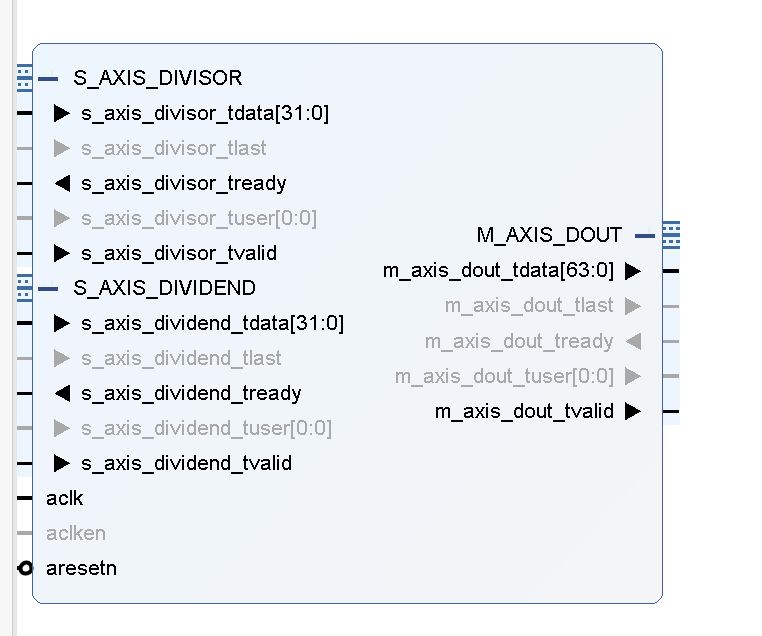
\includegraphics[width=0.6\linewidth]{Figures/fig1.png}
    \item \texttt{s\_axis\_dividend\_tdata} 对应计算时输入的被除数数据,\texttt{s\_axis\_divisor\_tdata} 对应计算时输入的除数数据,\texttt{m\_axis\_dout\_tdata} 中输出得到的商和余数,[63:32]位存放商,[31:0]存放余数。
    (上图中其他使用的信号,可能大家并不会完全用到,请根据自身使用情况进行调整,不需要跟途中的除法器配置完全保证一致,只需要保证功能可以正常实现即可)
\end{itemize}

对于两个输入通道和一个输出通道,除了有上述的数据信号外,每个通道都有一对 tvalid、
tready 信号。这是一对 “握手” 控制信号,其工作原理类似于我们在 CPU 流水线之间使用的
valid、allowin 信号。tvalid 是请求信号,tready 是应答信号。在时钟上升沿到来时,如果采样得
到 tvalid 和 tready 都等于 1,则请求发起方和接收方之间完成一次成功的握手。如果我们假想接收方有一组触发器缓存,那么所谓的成功握手是指发送方的数据写入接收方的缓存中,也就是在
握手成功的这个上升沿之后,触发器缓存会变为发送方的数据。

我们假设在执行流水阶段调用所生成的除法器 IP。在除法指令处于执行流水级且没有
对除法器成功输入数据的时候,同时将
\texttt{s\_axis\_dividend\_tvalid}和\texttt{s\_axis\_divisor\_tvalid}
置为 1。当发现 \texttt{s\_axis\_dividend\_tready} 和 \texttt{s\_axis\_divisor\_tready} 反馈为 1 后(此时在一
个时钟上升沿同时看到 tvalid 和 tready 为 1,表示握手成功),需要将 \texttt{s\_axis\_dividend\_tvalid} 和
\texttt{s\_axis\_divisor\_tvalid} 清 0,也就是确保握手成功的那个时钟上升沿之后的 \texttt{s\_axis\_dividend\_tvalid}
一定同时置为 1,那么这里生成的除法器 IP 反馈的 \texttt{s\_axis\_dividend\_tready} 和 \texttt{s\_axis\_divisor\_tready}
一定也同时置为 1。这里再次强调,被除数和除数输入的 tready 置起后(也就是握手成功后),
tvalid 一定要撤销,否则对于除法器 IP 来说,它会认为又有一个新的除法运算。

完成输入数据的握手之后,除法指令就需要在执行流水级等待除法器 IP 最终输出结果。当
\texttt{m\_axis\_dout\_tvalid} 置为 1 时,表示除法计算完成。此时除法指令就可以从 \texttt{m\_axis\_dout\_tdata}
上取出计算结果,进入流水线的后续阶段。由于前面我们将流控策略设置为 Non Blocking,因此
输出通道上不需要外部反馈 tready 信号,换言之,不管产生多少结果、什么时候产生,外部都要
能够及时处理。

控制信号调整:当执行流水阶段上是一条除法指令时,仅当除法运算部件返回结果完成的信号之后这一级流水的 \texttt{ready\_go} 才能置为有效。


\subsection{实现电路级的乘法器,除法器}

可以自行学习Booth编码和华莱士数实现乘法器,以及学习实现迭代除法器,这里不给出过多的介绍,有兴趣的同学可自行实现。

\subsection{实验要求}

\begin{itemize}
    \item 添加乘除运算类指令mul.w、mulh.w、mulh.wu、div.w、mod.w、div.wu、mod.wu,运行对应的func,要求成功通过仿真和上板验证。
\end{itemize}
\cleardoublepage

\section{异常和中断支持}

\foreword{
    风
}{
    伊夫·唐吉
}{
    我站在今天设想过去又幻想未来,过去和未来在今天随意交叉,因而过去和未来都刮着现在的风。
}{
    Figures/C10.jpg
}

\begin{center}
    \highlight{强调:本节内容请搭配手册使用}
\end{center}

关于异常和中断的概念,在这里不进行过多的阐述,在CPU设计的角度来看,
中断可以看成是一种特殊的异常,下文中统一使用异常来指代中断和异常。

异常处理的绝大部分工作是由异常处理程序(软件)的完成的,
但在异常处理的开始和结束阶段则是硬件需要考虑的,这正是本节中我们需要考虑的。

\paragraph{异常处理的开始阶段} 首先硬件需要判断异常的触发条件,随后硬件需要自动保存异常的类型,
触发异常的指令,地址等信息以用来给异常处理程序。此外,硬件需要保证跳转到异常处理程序的入口执行,
并且处于高特权等级。

\paragraph{异常结束阶段} 需要跳转回到发生异常的指令处重新开始执行,并且保证特权等级回到最初环境的特权等级。


\subsection{控制状态寄存器}

上面提到,异常需要进行软硬件的协同处理,所以难以避免的需要进行硬件逻辑电路和异常处理软件的信息交互。
为了保证精确异常的实现,LoongArch 指令系统中定义了一组独立的寄存器用于这类信息的交互,
统称为控制状态寄存器(Control Status Register,简称 CSR)。

在本节内容中需要实现,设计的异常和中断的处理来说,相关的CSR有:CRMD、PRMD、ECFG、ESTAT、
ERA、BADV、EENTRY、SAVE0$\sim$3、TID、TCFG、TVAL、TICLR。这些寄存器的详细定义请参看指令手册。

\subsection{异常产生的条件判断}

\subsubsection{处理器核内部判定接收到中断}

根据 LoongArch 指令系统的定义,每个处理器核内部可以记录 12 个线中断。
除去应用于多核场景下的核间中断目前暂不考虑,还包括 8 个硬中断、2 个软中断和 1 个定时器中断。

硬中断可以理解为处理器核上有八个中断输入引脚,中断信号通过这八个引脚输入。
ESTAT 控制状态寄存器 IS(Interrupt State)域的 9到2 这八位(RTL 上对应 8 个触发器)
则直接对中断输入引脚的信号采样。

软件中断顾名思义是由软件来设置的,通过 CSR 写指令对ESTAT 状态控制寄存器 IS 域的 1..0 
这两位写 1 或写 0 就可以完成两个软件中断的置起和撤销。

定时器中断的状态记录在 ESTAT 控制状态寄存器 IS 域的第 11 位。

从上面描述可知,ESTAT的IS域的11,9..0这11位记录了中断的11个状态,均为高电平表示有效。
但是处理器核中是否接受中断还需要看中断的使能情况,分为两个层次:

低层次-局部中断使能,由ECFG的LIE(local interrupt enable)域的11,9..0位依次对应控制

高层次-全局中断使能,通过CRMD的IE(interrupt enable)位来控制

综上可以给出处理器内部判断中断信号的\texttt{has\_int}可以这样实现:

\begin{lstlisting}
    assign has_int =  ((csr_estat_is[12:0] & csr_ecfg_lie[12:0]) != 13'b0)
    && (csr_crmd_ie == 1'b1);
\end{lstlisting}

注:在la32r中,不考虑多个中断的先后顺序,无论是接收到一个外部中断还是多个外部中断,此信号都可以被置为有效

\subsubsection{核内定时器中断的产生}

定时器中断经常用于操作系统的调度和计时功能的实现。该中断源来自于定时器,
通常分为核外和核内两种实现方式。LoongArch 指令系统采用了核内实现定时器中断源的方式。
简单来说,在每个 LoongArch32 处理器核内部实现一个 32 位的计数器,
在开启定时功能后每个时钟周期减1,当减到 0 值即可触发一次定时器中断。
接下来介绍其定义细节:
\begin{itemize}
    \item 定时器的软件配置集中在 TCFG(Timer Config)控制状态寄存器,包括它的启动使能
    、倒计时初始值和倒计时模式。其中倒计时模式分为两种,一种是减到 0 后即停止计数,另一种是减到 0 
    后自动装载倒计时初始值再次开始新一轮倒计时。
    \item 定时器的时钟与 \texttt{rdcntv{l/h}.w} 指令所访问的计时器使用同一时钟,这个时钟要求频率固定,
    我们尚不考虑处理器核的变频和关停,所以可以采用处理器核流水线的时钟。
    \item 定时器当前的计数值仅可以通过读取 TVAL 状态寄存器近似获得,它与 \texttt{rdcntv{l/h}.w} 
    指令读取的计时器值来自于两个截然不同的对象。
    \item 当定时器倒计时到 0 时硬件将 ESTAT 控制状态寄存器
     IS 域的第 11 位置 1,软件通过对 TICLR 控制寄存器的 CLR 位写 1 将 ESTAT 控制状态寄存器 
     IS 域的第 11 位清 0。
\end{itemize}


\subsubsection{取指地址错异常ADEF}

要求所有指令的PC都是字对齐的(地址最低两比特全为0),否则触发ADEF。

检测逻辑:对取指所用的 PC 的最低两位进行判断,如果不是 \texttt{2'b00} 的话,则置起取指地址错异常标志。
我们推荐在 pre-IF 级就进行这一判断。从严格意义上讲,出现异常的取指地址不应该用来发起取指的请求,
因为此时这个 PC 可能已经完全不正确,所以它的访存行为也不再软件人员的预想之内,最严重时可能导致死机等错误。

\subsubsection{地址非对齐异常ALE}

地址非对齐仅针对load,store这类的访存指令。当lh,lhu和sh指令的地址最低位不为0时,
或者lw,sw指令的地址最低两位不为全0时,触发ALE。

检测逻辑:需对 load、store 指令的地址进行判断,当访存地址出现非对齐情况时,
则置起地址非对齐异常标志。与前一节的设计思路一致,我们推荐在发起访存请求的EXE 级进行上述判断,
这样可以在发现异常情况的时候停止用错误地址发起访存请求。

\subsubsection{指令不存在异常INE}

当取回的指令码不属于任何一条已实现的指令时,将触发INE。

检测逻辑:可知指令不存在异常需要对指令译码后才得到检测结果。
由于我们需要在译码阶段对每一条实现的指令进行解码生成控制信号,
所以自然就可得到 ``不是任何一条实现的指令'' 的条件。

\subsubsection{系统调用SYS和断点异常BRK}

当执行 SYSCALL 指令时触发系统调用异常,当执行 BREAK 指令时触发断点异常。

检测逻辑:译码发现是syscall 指令就置起系统调用异常标志,译码发现 break 指令就置起断点异常标志。

\subsection{精确异常的实现}

为了实现精确异常,我们并不需要一发生异常就马上去修改控制状态寄存器和PC。
发生异常时仅需要考虑该如何处理那些在流水线中的指令。

这里给出一种处理思路:异常发生的判断逻辑分布在各流水级,
靠近与之相关的数据通路;发现异常后将异常信息附着在指令上沿流水线一路携带下去,
直至写回级才真正报出异常,此时才会根据所携带的异常信息更新控制状态寄存器;
写回指令报出异常的同时,清空所有流水级缓存的状态,并将 \texttt{nextPC} 置为异常入口地址。

当然不一定在写回级报出异常,但必须保证该级之后的流水级不能产生新的异常,否则这就不满足精确异常的要求。

\subsection{控制状态存储器的实现}

控制寄存器需要被\texttt{csrrd},\texttt{csrwr},\texttt{csrxchg}这样的CSR指令访问,
又需要和各级流水端口交互,看起来又集中又分散,下面给出一些设计的建议:

\begin{itemize}
    \item 把所有的控制状态寄存器集中到一个模块中实现;
    \item 模块接口分为用于指令访问的接口和与处理器核内部硬件电路逻辑直接交互的控制、状态信号接口两类;
    \item 指令访问接口包含读使能(\texttt{csr\_re})、寄存器号(\texttt{csr\_num})、
    寄存器读返回值(\texttt{csr\_rvalue})、写使能(\texttt{csr\_we})、写掩码(\texttt{csr\_wmask})和写数据(\texttt{csr\_wvalue});
    \item 与硬件电路逻辑直接交互的接口信号视需要各自独立定义,
    无须再统一编码,如送往预取指(pre-IF)流水级的异常处理入口地址 \texttt{ex\_entry}、
    送往译码流水级的中断有效信号 \texttt{has\_int}、来自写回流水级的 \texttt{ertn} 指令执行的有效信号 
    \texttt{ertn\_flush}、来自写回流水级的异常处理触发信号 \texttt{wb\_ex} 以及异常类型类型\texttt{wb\_ecode}、
    \texttt{wb\_esubcode} 等。
\end{itemize}

下面给出一个具体的CSR端口设计:

接下来给出每个域的具体分析和部分实现举例:

\subsubsection{CRMD 的 PLV 域}

从指令手册的定义可知 CRMD 的 PLV 域是可以通过 CSR 指令更新,而且在触发异常和 \texttt{ertn} 指令执行时也将被更新。

\begin{lstlisting}
    always @(posedge clock) begin
        if (reset)
            csr_crmd_plv <= 2'b0;
            else if (wb_ex)
            csr_crmd_plv <= 2'b0;
        else if (ertn_flush)
            csr_crmd_plv <= csr_prmd_pplv;
            else if (csr_we && csr_num==`CSR_CRMD)
            csr_crmd_plv <= csr_wmask[`CSR_CRMD_PLV]&csr_wvalue[`CSR_CRMD_PLV]
                            | ~csr_wmask[`CSR_CRMD_PLV]&csr_crmd_plv;
    end
\end{lstlisting}

这个代码应该是比较好理解的,
每一个写入条件和写入的值基本上都可以与指令手册中的定义一一对应上。
实现时,重点关注 CSR 模块的各个输入信号没有接错即可。

\subsubsection{CRMD的IE域}

\begin{lstlisting}
    always @(posedge clock) begin
        if (reset)
            csr_crmd_ie <= 1'b0;
        else if (wb_ex)
            csr_crmd_ie <= 1'b0;
        else if (ertn_flush)
            csr_crmd_ie <= csr_prmd_pie;
        else if (csr_we && csr_num==`CSR_CRMD)
            csr_crmd_ie <= csr_wmask[`CSR_CRMD_PIE]&csr_wvalue[`CSR_CRMD_PIE]
                        | ~csr_wmask[`CSR_CRMD_PIE]&csr_crmd_ie;
    end
\end{lstlisting}

请根据手册自行理解,对比CRMD的IE和PLV域的代码,可以发现就分支条件基本一样,代码处理操作也是相似的。

\subsubsection{CRMD 的 DA、PG、DATF、DATM 域}

目前我们设计的处理器还没有实现 MMU 的全部功能,仅支持直接地址翻译模式,所以
CRMD 的 DA、PG、DATF、DATM 域可以暂时置为常值。具体何值请根据手册自行判断。

\subsubsection{PRMD 的 PPLV、PIE 域}

\begin{lstlisting}
    always @(posedge clock) begin
        if (wb_ex) begin
            csr_prmd_pplv <= csr_crmd_plv;
            csr_prmd_pie <= csr_crmd_ie;
        end
    else if (csr_we && csr_num==`CSR_PRMD) begin
        csr_prmd_pplv <= csr_wmask[`CSR_PRMD_PPLV]&csr_wvalue[`CSR_PRMD_PPLV]
                        | ~csr_wmask[`CSR_PRMD_PPLV]&csr_prmd_pplv;
        csr_prmd_pie <= csr_wmask[`CSR_PRMD_PIE]&csr_wvalue[`CSR_PRMD_PIE]
                        | ~csr_wmask[`CSR_PRMD_PIE]&csr_prmd_pie;
        end
    end
\end{lstlisting}

\subsubsection{ECFG 的 LIE 域}

请根据手册和上面示例代码自行实现

\subsubsection{ESTAT 的 IS 域}

ESTAT 的 IS 域中,1..0 位、9..2 位、11 位、12 位的更新来源存在区别,其依次仅被 CSR
指令更新、仅通过采样处理器核硬件中断输入引脚更新、仅根据定时器计数器和 TICLR.CLR 域
的写更新、仅通过采样处理器核的核间中断输入引脚更新。第 10 位没有定义,保险起见我们将
其恒置为 0。

\begin{lstlisting}
    always @(posedge clock) begin
        if (reset)
            csr_estat_is[1:0] <= 2'b0;
        else if (csr_we && csr_num==`CSR_ESTAT)
            csr_estat_is[1:0] <= csr_wmask[`CSR_ESTAT_IS10]&csr_wvalue[`CSR_ESTAT_IS10]
                            | ~csr_wmask[`CSR_ESTAT_IS10]&csr_estat_is[1:0];

        csr_estat_is[9:2] <= hw_int_in[7:0];

        csr_estat_is[10] <= 1'b0;

        if (timer_cnt[31:0]==32'b0)
            csr_estat_is[11] <= 1'b1;
        else if (csr_we && csr_num==`CSR_TICLR && csr_wmask[`CSR_TICLR_CLR]
                && csr_wvalue[`CSR_TICLR_CLR])
            csr_estat_is[11] <= 1'b0;

        csr_estat_is[12] <= ipi_int_in;

    end
\end{lstlisting}

\subsubsection{ESTAT 的 Ecode 和 EsubCode 域}

ESTAT 的 Ecode 和 EsubCode 域需要在触发异常时填入异常的类型代号。
见手册,我们推荐采用每个异常单独一个标志信号的传递方式,
最后在写回级编码为 Ecode 和 EsubCode 值送到 CSR 模块。

\begin{lstlisting}
    always @(posedge clock) begin
        if (wb_ex) begin
            csr_estat_ecode <= wb_ecode;
            csr_estat_esubcode <= wb_esubcode;
        end
    end
\end{lstlisting}

\subsubsection{ERA 的 PC 域}

当位于写回级指令触发异常时,需要记录到 ERA 寄存器的 PC 就是当前写回级的 PC。
根据手册和以上示例代码自行实现

\subsubsection{BADV 的 VAddr 域}

BADV 的 VAddr 域和 ERA 的 PC 域的维护有相似之处,都是在写回级指令触发异常时,记录该指令的一些信息。

这里需要注意一点,在支持异常处理之前,处理器流水线中在访存级和写回级是不需要保存
 load,store 指令完整的虚地址的。但是为了BADV的VAddr域的正常维护,我们需要在流水线中进行保存。

根据手册和以上示例代码自行实现

\subsubsection{EENTRY 的 VA 域}

根据手册和以上示例代码自行实现

\subsubsection{SAVE0$\sim$3}

SAVE0$\sim$3 就是提供给特权态软件临时存放数值用的,给出部分示例实现,自行补全完整

\begin{lstlisting}
    always @(posedge clock) begin
        if (csr_we && csr_num==`CSR_SAVE0)
            csr_save0_data <= csr_wmask[`CSR_SAVE_DATA]&csr_wvalue[`CSR_SAVE_DATA]
                            | ~csr_wmask[`CSR_SAVE_DATA]&csr_save0_data;
        if (csr_we && csr_num==`CSR_SAVE1)
            csr_save1_data <= csr_wmask[`CSR_SAVE_DATA]&csr_wvalue[`CSR_SAVE_DATA]
                            | ~csr_wmask[`CSR_SAVE_DATA]&csr_save1_data;
    end
\end{lstlisting}

\subsubsection{TID}

TID 寄存器的维护也是比较简单的,根据手册和示例自行实现

\subsubsection{TCFG 的 En、Periodic 和 InitVal 域}

根据手册和示例自行实现

\subsubsection{TVAL 的 TimeVal 域}

TVAL 的 TimeVal 域是一个软件只读域,它返回定时器计数器的值即可,所以可以将其实现
为 wire 而非 reg。此处的设计关键点在于用作定时器的计数器 \texttt{timer\_cnt} 的实现。

\begin{lstlisting}
    reg csr_tcfg_en;
    reg csr_tcfg_periodic;
    reg [29:0] csr_tcfg_initval;
    wire [31:0] tcfg_next_value;
    wire [31:0] csr_tval;

    reg [31:0] timer_cnt;
    assign tcfg_next_value = csr_wmask  [31:0]&csr_wvalue[31:0]
                            | ~csr_wmask[31:0]&{csr_tcfg_initval,
                                                csr_tcfg_periodic, csr_tcfg_en};

    always @(posedge clock) begin
        if (reset)
            timer_cnt <= 32'hffffffff;
        else if (csr_we && csr_num==`CSR_TCFG && tcfg_next_value[`CSR_TCFG_EN])
            timer_cnt <= {tcfg_next_value[`CSR_TCFG_INITVAL], 2'b0};
        else if (csr_tcfg_en && timer_cnt!=32'hffffffff) begin
            if (timer_cnt[31:0]==32'b0 && csr_tcfg_periodic)
                timer_cnt <= {csr_tcfg_initval, 2'b0};
            else
                timer_cnt <= timer_cnt - 1'b1;
        end
    end

    assign csr_tval = timer_cn[31:0];      
\end{lstlisting}

\begin{itemize}
    \item 我们在软件对 timer 进行配置(也就是更新 TCFG 控制状态寄存器的时候)的同时发起
    \texttt{timer\_cnt} 的更新操作。具体来说,就是当软件开启 timer 的使能时(即将 TCFG 的 En 域
    置 1),将此时写入的 timer 配置寄存器的定时器初始值更新到 \texttt{timer\_cnt} 中;当软件关闭
    timer 的使能时,\texttt{timer\_cnt} 不更新。因为是在软件写 TCFG 的同时更新 timer,所以要看
    当前写入 TCFG 寄存器的值(\texttt{tcfg\_next\_value}),而不是用 TCFG 寄存器已有的值。
    \item 当 \texttt{timer\_cnt} 减到全 0 且定时器不是周期性工作模式的情况下,代码中没有专门处理的逻
    辑,所以 \texttt{timer\_cnt} 会继续减 1 变成 \texttt{32'hffffffff}。不过,因为此时定时器是非周期性的,所
    以它应该停止计数,这就是为何 \texttt{timer\_cnt} 自减的使能条件除了看 \texttt{csr\_tcfg\_en} 是否为 1
    外还会看 \texttt{tmer\_cnt}!=\texttt{32'hffffffff} 这个条件         
\end{itemize}

\subsubsection{TICLR 的 CLR 域}

TICLR 的 CLR 域很特殊,它的读写属性是 ``W1'',意味着软件只有对它写 1 才会产生执行
效果(即硬件只捕获对 TICLR 的 CLR 域写 1 这个动作),写 0 无效,同时软件读出的值永远
是 0。所以,TICLR 的 CLR 域并不需要定义一个 reg 与之对应,我们只需要定义一个恒为 0 的
wire 用于后面的 CSR 读出即可。

\subsubsection{CSR 的读出}

给出示例如:

\begin{lstlisting}
    wire [31:0] csr_prmd_rvalue = {29'b0, csr_prmd_pie, csr_prmd_pplv};
    wire [31:0] csr_ecfg_rvalue = {19'b0, csr_ecfg_lie};

    assign csr_rvalue = {32{csr_num==`CSR_CRMD}} & csr_crmd_rvalue
                      | {32{csr_num==`CSR_PRMD}} & csr_prmd_rvalue
\end{lstlisting}


\subsection{相关冲突的处理}

最经典的CSR写后读相关是\texttt{csrwr}或者\texttt{csrxchg}这两个指令修改一个CSR后又有\texttt{csrrd},
\texttt{csrwr}或者\texttt{csrxchg}指令读取同一个CSR,为了解决这种冲突,最简单有效的方法就是将所有的CSR读
写指令访问CSR的操作都放到同一流水级进行处理,虽然会损失一些性能,但是影响并不是很大。

\begin{table}[H]
    \centering
    \begin{adjustbox}{width=\linewidth} 
    \small
    \begin{tabularx}{\linewidth}{ccc}
        \toprule
        {\bfseries 写者} & {\bfseries 相关对象} & {\bfseries 读者} \\ 
        \midrule
        \multirow{2}{*}{csrwr 或 csrxchg} & CRMD.IE、ECFG.LIE、ECFG.IS[1:0]、TCFG.En、TICLR.CLR& 译码级的指令(标记中断)\\
         & ERA、PRMD.PPLV、PRMD.PIE& ertn\\
        \multirow{2}{*}{ertn} & CRMD.IE&译码级的指令 \\
         &CRMD.PLV &取指的 PC \\
        \bottomrule
    \end{tabularx}
\end{adjustbox}
\end{table}

我们这里处理冲突最主要的还是用阻塞,并不考虑前递。

前面三种情况的的阻塞仍是直截了当,只需要判断EXE,MEM,WB级的时候有没有这几种情况的写相关性的写者
,如果有就直接阻塞(阻塞在译码级)。

第四种情况,在流水线中最早只能在译码的时候能知道写者和相关对象,
但是这个时候取值级已经取出来一个指令了,现在单靠阻塞是不能解决问题了,
这里给出一种特殊的处理方法:\texttt{ertn} 指令直到写回级才修改 CRMD,与
此同时清空流水线并更新取指 PC。这也就是前面提到的 \texttt{ertn\_flush} 信号的由来。

\subsection{实验要求}

\begin{itemize}
    \item 为 CPU 增加 csrrd、csrwr、csrxchg 和 ertn 指令
    \item 为 CPU 增加控制状态寄存器 CRMD、PRMD、ESTAT、ERA、EENTRY、SAVE0$\sim$3。
    \item 为 CPU 增加 syscall 指令,实现系统调用异常支持。
    \item 运行对应的 func,要求成功通过仿真和上板验证。
\end{itemize}

\begin{itemize}
    \item 为CPU 增加取指地址错(ADEF)、地址非对齐(ALE)、断点(BRK)和指令不存在(INE)
    异常的支持。
    \item 为 CPU 增加中断的支持,包括 2 个软件中断、8 个硬件中断和定时器中断。
    \item 为 CPU 增加 rdcntvl.w、rdcntvh.w 和 rdcntid 指令。
    \item 为 CPU 增加控制状态寄存器 ECFG、BADV、TID、TCFG、TVAL、TICLR。
    \item 运行对应的func,要求成功通过仿真和上板验证。
\end{itemize}


\cleardoublepage

\section{结语} \label{section: conclusion}

\textcolor{Ustb-blue}{\textbf{希望大家能感受,享受来自数字逻辑的魅力。}}

\cleardoublepage

% %Creates references using the Biblatex
% %    \bibliographystyle{plain}
% %    \bibliography{General/References.bib}
% %   \cleardoublepage

\appendix  % Any section after this command will have a letter as an index

% % Adds an appendix entry
\section{LA组评分细则}

\subsection{任务要求}

\subsubsection{写在开头}

\highlight{个人任务需要个人独立完成验收,创新扩展部分在答辩环节进行展示,需要在答辩中展示创新扩展的正确性。}

\begin{itemize}
    \item 关于答辩会提的问题:
    \begin{itemize}
        \item 主要会围绕着创新内容部分进行考察,考察原理和实现思路。
    \end{itemize}
    \item 关于评分与难度的非线性关系:
    \begin{itemize}
        \item 之所以存在这种非线性关系,主要是为了一般的同学能够拿到分数,对此感兴趣的同学可以深入。不喜欢这个方向就没必要卷计组课设了,抓紧时间学好其他专业课。
    \end{itemize}
    \item 关于分数分布
    \begin{itemize}
        \item 本课程的总分100分,难度最大的部分其实在创新扩展部分,而其他的部分都只要认真把握课程原理,即可实现,请同学们重点把握这部分知识,充分理解;
        \item 不建议大家死磕创新扩展的实现,\highlight{更禁止通过抄袭的方式获得这一部分分数},请大家实事求是。
    \end{itemize}
\end{itemize}

\subsubsection{个人任务 60分}

根据给出的实验指导书完成前五个章节:

\begin{itemize}
    \item 不考虑冲突的简单五级流水划分;
    \item 指令相关和流水线冲突;
    \item 算术逻辑转移类指令的添加;
    \item 访存指令的添加;
    \item 乘除法指令的添加。
\end{itemize}

\paragraph{实验报告——个人部分 10分}

\subsubsection{团队任务 40分}

\paragraph{创新基础部分}

异常相关指令扩展 (根据指导书的最后一章,实现异常和中断的支持):

\begin{itemize}
    \item 第一阶段:
    \begin{itemize}
        \item 增加 csrrd、csrwr、csrxchg 和 ertn 指令;
        \item 为 CPU 增加控制状态寄存器 CRMD、PRMD、ESTAT、ERA、EENTRY、SAVE0-3;
        \item 为 CPU 增加 syscall 指令,实现系统调用异常支持。
    \end{itemize}
    \item 第二阶段:
    \begin{itemize}
        \item 增加取指地址错(ADEF)、地址非对齐(ALE)、断点(BRK)和指令不存在(INE)异常的支持;
        \item 增加中断的支持,包括 2 个软件中断、8 个硬件中断和定时器中断;
        \item 增加 rdcntvl.w、rdcntvh.w 和 rdcntid 指令;
        \item 增加控制状态寄存器 ECFG、BADV、TID、TCFG、TVAL、TICLR。
    \end{itemize}
\end{itemize}

\paragraph{创新扩展部分}

给出多个选项参考,并不需要大家全部完成,如有其他自行设计的创新扩展不在本范围内也可。

\begin{itemize}
    \item AXI总线接口设计:
    \begin{itemize}
        \item 将CPU顶层接口修改为AXI总线接口。
    \end{itemize}
    \item 缓存模块设计:
    
    Cache是现代计算机中不可缺少的技术。

    \begin{itemize}
        \item Cache基本实现为一路直接映射Cache,二者都实现时取DataCache成绩;
        \item Cache指令实现;
        \item 多路组相连Cache;
        \item Cache流水化。
    \end{itemize}
    \item 外设功能扩展
    \begin{itemize}
        \item 通过汇编语言代码对SoC上已经提供实现了的外设进行操控;
        \item 集成串口外设,并能通过汇编语言代码操纵外设。
    \end{itemize}
\end{itemize}

\paragraph{实验报告——团队部分 10分}




\cleardoublepage

\section{MIPS组评分细则}

\subsection{任务要求}

\subsubsection{写在开头}

\highlight{个人任务需要个人独立完成验收,创新扩展部分在答辩环节进行展示,需要在答辩中展示创新扩展的正确性。}

\begin{itemize}
    \item 关于答辩会提的问题:
    \begin{itemize}
        \item 主要会围绕着创新内容部分进行考察,考察原理和实现思路。
    \end{itemize}
    \item 关于评分与难度的非线性关系:
    \begin{itemize}
        \item 之所以存在这种非线性关系,主要是为了一般的同学能够拿到分数,对此感兴趣的同学可以深入。不喜欢这个方向就没必要卷计组课设了,抓紧时间学好其他专业课。
    \end{itemize}
    \item 关于分数分布
    \begin{itemize}
        \item 本课程的总分100分,难度最大的部分其实在创新扩展部分,而其他的部分都只要认真把握课程原理,即可实现,请同学们重点把握这部分知识,充分理解;
        \item 不建议大家死磕创新扩展的实现,\highlight{更禁止通过抄袭的方式获得这一部分分数},请大家实事求是。
    \end{itemize}
\end{itemize}

\subsubsection{个人任务 60分}

\paragraph{CG 测评任务 20分}

完成CG上评测题,需要提交的代码已经在CDE工程中给出。请阅读实验指导书《计算机组成原理课程设计实验指导书 下》,学习TinyMIPS的基本结构。并提交相应代码。

\paragraph{虚拟仿真实验平台 10分}

\begin{itemize}
    \item 完成虚拟仿真实验平台上的四个实验。包括模拟器运行和代码运行;
    \item 本部分实验重点在于解决流水线的前递与暂停问题,与实验指导书的第二章结尾和第三章结尾有关。请注意体会其原理,在进行乘除法器的扩展过程中,同样需要利用到前递和暂停的知识。
\end{itemize}

\paragraph{扩展指令任务 20分}

\begin{itemize}
    \item 要求选择TinyMIPS CPU中未扩展的22条指令中的若干条进行扩展,具体包含的指令在表~\ref{tab: x1},对于ADD,SUB等涉及异常的指令,暂时可以不用扩展异常处理的内容。
    \item 对于每一条指令,都有若干其所属的分组和一个基础分值。
    \item 每个指令的基础分值根据扩展该指令时的工作量进行设置,具体见表~\ref{tab: x1}。
    \item 如果选择了多条同分组的指令,自第二条起,其计算分值减少为基础分值的1/2。
    \item 要求最终同学们完成计算分值总计10分的指令扩展。多做不加分。
    \item 个人任务需要到现场进行验收,演示对指令的测试过程。验收现场会进行提问,提问内容不仅涉及下面的指令扩展的思路过程,也包括Trace机制,测试用例,MIPS指令集架构相关的知识。
\end{itemize}


\begin{table}
    \centering
    \caption{指令分值}\label{tab: x1}
    \begin{tabular}{cccc}
        \toprule
        {\bfseries 序号} &  {\bfseries 指令名称} &  {\bfseries 指令分值} &  {\bfseries 指令分组}\\ 
        \midrule
        1       &   ADD     &   2       &       R型运算指令/加法指令        \\
        2       &   SUB     &   2       &       R型运算指令     \\
        3       &   NOR     &   2       &       R型运算指令     \\
        4       &   ADDI    &  2        &       I型运算指令/加法指令        \\
        5       &   ANDI    &  2        &       I型运算指令     \\
        6       &   ORI     &   2       &       I型运算指令     \\
        7       &   XORI    &  2        &       I型运算指令     \\
        8       &   SLTI    &  2        &       I型运算指令     \\
        9       &   SLTIU   &     2     &       I型运算指令     \\
        10      &   SRL     &   2       &       Shamt移位指令       \\
        11      &   SRA     &   2       &       Shamt移位指令       \\
        12      &   J   &     2     &       直接跳转指令        \\
        13      &   JR  &    3      &       直接跳转指令        \\
        14      &   LH  &    3      &       内存载入指令        \\
        15      &   LHU     &   3       &       内存载入指令        \\
        16      &   SH  &    3      &       内存存储指令        \\
        17      &   BGEZ    &  3        &       条件分支指令/BGE跳转        \\
        18      &   BGTZ    &  3        &       条件分支指令        \\
        19      &   BLEZ    &  3        &       条件分支指令        \\
        20      &   BLTZ    &  3        &       条件分支指令/BLT跳转        \\
        21      &   BGEZAL  &    3      &       条件分支指令/BGE跳转        \\
        22      &   BLTZAL  &    3      &       条件分支指令/BLT跳转        \\
        \bottomrule
    \end{tabular}
\end{table}

例如一个同学选择了ADD指令,ORI指令,ANDI指令,JR指令,LH指令,其总分值为2,2,1,3,3 共计 11分,可以达到验收要求。

\paragraph{实验报告——个人部分 10分}

\subsubsection{团队任务 40分}

\paragraph{创新基础部分}

创新部分基础实现包括《计算机组成原理课程设计指导书补充内容》所介绍的全部内容:

\begin{itemize}
    \item 乘除法指令扩展:
    \begin{itemize}
        \item 通过乘除法测试点,包括\texttt{n44\_div},\texttt{n45\_divu},\texttt{n46\_mult},\texttt{n47\_multu},\texttt{n48\_mfhi},\texttt{n49\_mflo},\texttt{n50\_mthi},\texttt{n51\_mflo};
        \item 乘除法模块可以采用IP核实现。
    \end{itemize}
    \item 异常相关指令扩展:
    \begin{itemize}
        \item 第一阶段:
        \begin{itemize}
            \item 实现特权指令\texttt{ERET},\texttt{MTC0},\texttt{MFC0}
            \item 自陷指令\texttt{BREAK},\texttt{SYSCALL}
            \item 实现A02文件中规定的所有CP0寄存器
        \end{itemize}
        \item 第二阶段:
        \begin{itemize}
            \item 继续扩展异常,通过完整89个功能点的测试
        \end{itemize}
    \end{itemize}
\end{itemize}

\paragraph{创新扩展部分}

给出多个选项参考,并不需要大家全部完成,如有其他自行设计的创新扩展不在本范围内也可。

\begin{itemize}
    \item 缓存模块设计:
    
    Cache是现代计算机中不可缺少的技术。

    \begin{itemize}
        \item Cache基本实现为一路直接映射Cache,二者都实现时取DataCache成绩;
        \item Cache指令实现;
        \item 多路组相连Cache;
        \item Cache流水化。
    \end{itemize}
    \item 外设功能扩展
    \begin{itemize}
        \item 通过汇编语言代码对SoC上已经提供实现了的外设进行操控;
        \item 集成串口外设,并能通过汇编语言代码操纵外设。
    \end{itemize}
\end{itemize}

\paragraph{实验报告——团队部分 10分}




\cleardoublepage

%%%
\end{document}
